\chapter{Additional informations on computation}
\label{appendix:add_info}
\section{Element-wise product}
\label{appendix:add_info_element_wise_product}
The element-wise product between two matrix $\mathbf{A}$ and $\mathbf{B}$ is noted $\mathbf{A} \odot \mathbf{B}$ and is defined in the following way:\\
For two matrices $\mathbf{A}$, $\mathbf{B}$ of same dimensions $n \times m$, the element-wise product is a $n \times m$ matrix where the elements are defined by:
\[(\mathbf{A} \odot \mathbf{B})_{i,j} = (\mathbf{A})_{i,j} \cdot (\mathbf{B})_{i,j}\]
The product is undefined for matrices of different dimensions

\section{Kronecker product}
\label{appendix:add_info_kronecker_product}
The Kronecker product of two matrix $\mathbf{A}$ and $\mathbf{B}$ of respective dimensions $n \times m$ and $p \times q$ is a $np \times mq$ block matrix where the elements are defined by:
\[\mathbf { A } \otimes \mathbf { B } = 
\left[ 
\begin{array}
 { c c c } { a _ { 11 } \mathbf { B } } & { \cdots } & { a _ { 1 n } \mathbf { B } } \\ { \vdots } & { \ddots } & { \vdots } \\ { a _ { m 1 } \mathbf { B } } & { \cdots } & { a _ { m n } \mathbf { B } } 
\end{array} 
\right]\] 

\section{Polynomials splines}
\label{appendix:polynomial_splines}
\textcite{fahrmeir_regression:_2013} state that a function $f : [ a , b ] \rightarrow \mathbb { R }$ is called a polynomial spline of degree $l \geq 0$ with knots $a = \kappa _ { 1 } < \ldots < \kappa _ { m } = b$, if it fulfills the following conditions:
\begin{enumerate}
\item $f(z)$ is $(l-1)$ times continuously differentiable. The special case of $l = 1$ corresponds to $f(z)$ being continuous (but not differentiable). We do not state any smoothness requirements for $f(z)$ when $l=0$.
\item $f(z)$ is a polynomial of degree $l$ on intervals $\left[ \kappa _ { j } , \kappa _ { j + 1 } \right)$ defined by the knots.
\end{enumerate}
Moreover, it can be shown that each polynomial spline of degree $l$ with
knots $\kappa _ { 1 } < \ldots < \kappa _ { m }$ can be uniquely determined as a linear combination of the $d = l+m-1$ functions
$B_1, \dots , B_d$, called the \textit{basis functions}, since we can uniquely represent all polynomials splines by using these functions.

\subsection{B-splines}
B-splines are polynomial splines with specific basis functions. B-spline basis functions are constructed
from piecewise polynomials that are fused smoothly at the knots to achieve the desired smoothness constraints. More specifically, a B-spline basis function consists
of $(l+1)$ polynomial pieces of degree $l$ , which are joined in an $(l-1)$ continuously differentiable way. All B-spline basis functions are set up based on a given knot configuration. Using the complete basis, the function $f(z)$ can again be represented through a linear combination of $d = m + l-1$ basis
functions, i.e.,
\[f ( z ) = \sum _ { j = 1 } ^ { d } \gamma _ { j } B _ { j } ( z )\text{.}\]
The B-splines of order $l=0$ can be written as
\[B _ { j } ^ { 0 } ( z ) = \left\{ \begin{array} { l l } { 1 } & { \kappa _ { j } \leq z < \kappa _ { j + 1 } } \\ { 0 } & { \text { otherwise } } \end{array} \right. \quad j = 1 , \ldots , d - 1\]
and the B-splines for higher order $l$ can be written as
\[B _ { j } ^ { l } ( z ) = \frac { z - \kappa _ { j - l } } { \kappa _ { j } - \kappa _ { j - l } } B _ { j - 1 } ^ { l - 1 } ( z ) + \frac { \kappa _ { j + 1 } - z } { \kappa _ { j + 1 } - \kappa _ { j + 1 - l } } B _ { j } ^ { l - 1 } ( z ) \text{.}\]
The estimation of a polynomial spline in B-spline representation can be traced back to the estimation of a linear model with a large number of parameters and design matrix 
\[\mathbf{Z}= \left( \begin{array} { c c c } { B _ { 1 } ^ { l } \left( z _ { 1 } \right) } & { \dots } & { B _ { d } ^ { l } \left( z _ { 1 } \right) } \\ { \vdots } & { } & { \vdots } \\ { B _ { 1 } ^ { l } \left( z _ { n } \right) } & { \dots } & { B _ { d } ^ { l } \left( z _ { n } \right) } \end{array} \right) \text{.} \]
The linear combination of basis functions can then be written in matrix form
\[ \mathbf{y} = \mathbf{Z} \mbox{\boldmath$\gamma$} \]
where the coefficient matrix, {\boldmath$\gamma$} can be estimated using least squares.\\
The estimation of a B-spline fit can be summarized in three steps:
\begin{enumerate}
\item We calculate a complete B-spline basis for a given number of knots.
\item The least squares estimate {\boldmath$\hat{\gamma}$} yields an amplitude $\hat{\gamma_j}$ for the scaling of every basis function.
\item We obtain the final estimate by summing the scaled basis function.
\end{enumerate}

\subsection{Penalized splines}
We clearly see that the quality of the estimation by polynomials splines highly depends on the number of knots and that this can easily lead to an over-fitting issue. To overcome this problem, \textit{penalized splines (P-splines)} introduce a roughness penalty term that prevents over-fitting and minimize a \textit{penalized least squares (PLS) criterion} instead of the usual least squares criterion.\\
To characterize the smoothness of any type of function, the
use of (squared) derivatives is appropriate, since these represent measures for the variability of a function. Therefore penalties based on the second derivative, such as
\[ \lambda \int \left( f ^ { \prime \prime } ( z ) \right) ^ { 2 } d z\text{,} \]
are particularly attractive since they measure the curvature of a function. Since we know that the first derivative of a B-spline can be written as a function of the first differences of the corresponding coefficient vector, we can use differences of a higher order $r$ if we aim at a smooth function in terms of $r$th-order derivatives. This leads to the penalized residual sum of squares
\[\operatorname { PLS } ( \lambda ) = \sum _ { i = 1 } ^ { n } \left( y _ { i } - \sum _ { j = 1 } ^ { d } \gamma _ { j } B _ { j } \left( z _ { i } \right) \right) ^ { 2 } + \lambda \sum _ { j = r + 1 } ^ { d } \left( \Delta ^ { r } \gamma _ { j } \right) ^ { 2 }\text{,}\]
where $\Delta^r$ denotes the $r$th-order differences.The smoothing parameter $\lambda \geq 0$ controls the compromise between fidelity to the data and smoothness of the resulting function estimate. The PLS criterion can be rewritten using matrix notation
\[ \operatorname { PLS } ( \lambda ) = ( \mathbf{y} - \mathbf{Z} \boldsymbol{\gamma} ) ^ { \prime } (  \mathbf{y} - \mathbf{Z} \boldsymbol{\gamma}) + \lambda \boldsymbol{\gamma} ^ { \prime }\mathbf{K_r} \boldsymbol{\gamma} \]
where $\mathbf{K_r}$ is the $r$th-order difference penalty matrix, and can be decomposed as $\mathbf{D_r}\prime \mathbf{D_r}$ with $D_r$ the $r$th-order difference matrix.
The smoothing parameter $\lambda \geq 0$ controls the compromise between fidelity to the data and smoothness of the resulting function estimate. The PLS estimate of the coefficient matrix is then 
\[ \hat { \boldsymbol{\gamma} } = \left(\mathbf{ Z} ^ { \prime } \mathbf {Z} + \lambda \mathbf{K} \right) ^ { - 1 }\mathbf{ Z} ^ { \prime }\mathbf{ y} \text{.}\]
For more detailed information about polynomials splines, please refer to \textcite{fahrmeir_regression:_2013} and \textcite{eilers_flexible_1996}

\section{Penalized form of the solution and smoothing parameter selection}
\label{appendix:SpATS_add_comput_info}
Let us consider the model only containing a bivariate smooth surface and an error term:
\[
	    y _ { i } = f \left( u _ { i } , v _ { i } \right) + \varepsilon _ { i } , \text { with } \varepsilon _ { i } \sim N 
	    \left( 0 , \sigma ^ { 2 } \right) \text{.} 
	    \]
It can be rewritten, in matrix notation, as the tensor product of B-splines:
\[
    \boldsymbol{y} = \boldsymbol{B}\boldsymbol{\alpha} + \boldsymbol{\epsilon}
    \text{.}
\]
Since the model is purely parametric, it can be estimated by minimizing the residual sum of squares (with explicit solution $\Hat{\boldsymbol{\alpha}} = (\mathbf{B}^t\mathbf{B})^{-1}\mathbf{B}^t\mathbf{y}$). To prevent over-fitting, \textcite{eilers_flexible_1996} propose to incorporate a discrete penalty on the coefficient associated to adjacent B-splines. For the two-dimensional case, the vector $\boldsymbol{\alpha}$ can be seen as an  $(L \times P)$  matrix  of  coefficients, $\mathbf{A}=[\alpha_{lp}]$. Now the rows  and columns of $\mathbf{A}$ correspond to the regression coefficients in the $v$ and  $u$ direction, respectively. In anisotropic (direction-dependant) P-splines, a different amount of smoothing is assumed along the $u$ and $v$ directions. It leads to two penalties:  one on all rows of $\mathbf{A}$,  the other on all of its columns; and the penalized least squares objective function becomes \parencite{eilers_multivariate_2003}
\[
\begin{aligned}
    S^{*} & = \underbrace{\|\boldsymbol{y}-\boldsymbol{B} \boldsymbol{\alpha}\|^{2}}_{\text{Original objective function}} \\
    	  & +\underbrace{\invbreve{\lambda}\|\invbreve{\boldsymbol{D}} A\|_{F}^{2}}_{\text{Penalty along the columns}} \\
    	  & +\underbrace{\breve{\lambda}\left\|\boldsymbol{A} \breve{D}^{t}\right\|_{F}^{2}}_{\text{Penalty along the rows}} \\
    =	  & \|\boldsymbol{y}-\boldsymbol{B} \boldsymbol{\alpha}\|^{2}+\boldsymbol{\alpha}^{t} \boldsymbol{P} \boldsymbol{\alpha}
    \text{,}
\end{aligned}
\]
where $\boldsymbol{P}=\invbreve{\lambda}\left(\boldsymbol{I}_{P} \otimes \invbreve{\boldsymbol{D}}^{t} \invbreve{\boldsymbol{D}}\right)+\breve{\lambda}\left(\breve{\boldsymbol{D}}^{t} \breve{\boldsymbol{D}} \otimes \boldsymbol{I}_{L}\right)$ is the penalty matrix, $\invbreve{\lambda}$ and $\breve{\lambda}$ are the smoothing parameters acting, respectively, on the columns and rows of $\mathbf{A}$, and $\invbreve{\mathbf{D}}$ and $\breve{\mathbf{D}}$ are the matrices that form differences of order $d_u$ and $d_v$ respectively. The minimizer of \ref{eq:least_squares_penalized} then becomes 
\[
    \widehat{\boldsymbol{\alpha}}=\left(\boldsymbol{B}^{t} \boldsymbol{B}+\boldsymbol{P}\right)^{-1} \boldsymbol{B}^{t} 
    \boldsymbol{y}
    \text{,}
\]
which is the penalized form of the solution. However, $\boldsymbol{P}$ is rank-deficient.
To have a full rank penalty matrix, the key is to rewrite the model and setting
\[
    \mathbf{B}\boldsymbol{\alpha} = \boldsymbol{X}_{s} \boldsymbol{\beta}_{s}+\boldsymbol{Z}_{s} \boldsymbol{c}_{s}
    \text{.}
\]
There are now two bases: $\mathbf{X}_{s}$, with coefficients that are not penalized at all, and $\mathbf{Z}_{s}$, with a size 
penalty on its coefficients. This decomposition follows the proposal by \textcite{lee_p-spline_2011}, based on eigenvalue 
decomposition which gives rise to a diagonal penalty matrix.\\

The two bases have the following structures:
\begin{equation*}
\boldsymbol{X}_{s}=\left[\mathbf{1}_{n}, \boldsymbol{u}, \boldsymbol{v}, \boldsymbol{u} \odot \boldsymbol{v}\right]
    \quad
    \text{and}
    \quad
    \mathbf{Z}_{s}=\left[\mathbf{Z}_{v}, \mathbf{Z}_{u}, \mathbf{Z}_{v} \boxdot \mathbf{u}, \mathbf{v} \boxdot \mathbf{Z}_{u}, 
    \mathbf{Z}_{v} \boxdot \mathbf{Z}_{u} \right]
    \text{,}
\end{equation*}
where $\boldsymbol{u}$ and $\boldsymbol{v}$ are still, respectively, the vectors of row and column positions. 
Here $\mathbf{Z}_{u}$ and $\mathbf{Z}_{v}$ are penalized version of the B-splines basis $\breve{\mathbf{B}}$ (rows) and
$\invbreve{\mathbf{B}}$ (columns). This new way of writing the problem leads to another penalty matrix 
$ \widetilde{\boldsymbol{P}}$, which is a block diagonal matrix. Each block of $ \widetilde{\boldsymbol{P}}$ corresponds to a 
block in $\mathbf{Z}_{s}$. Similarly to $\boldsymbol{P}$, the penalty matrix of the previous section, this new penalty matrix 
only depends on the two tuning parameters $\invbreve{\lambda}$ (smoothing along the columns) and $\breve{\lambda}$ (smoothing 
along the rows).
Figure \ref{fig:matrix_diagram} presents a diagram clarifying the structures and relations of the different matrices presented 
throughout this section.\\

This reformulation provides the ANOVA type decomposition discussed in the previous section 
(\ref{eq:full_bivariate_smooth_surface_model}), and explains how the bilinear smooth surface can be modelled using P-splines and 
tensor products of P-splines.
The block structure of $\mathbf{X}_s$ and $\mathbf{Z}_s$ implies
\[
    \begin{aligned} 
        f(\boldsymbol{u}, \boldsymbol{v}) & =\boldsymbol{X}_{s} \boldsymbol{\beta}_{s}+Z_{s} \boldsymbol{c}_{s} \\ 
        								  & =\mathbf{1}_{n} \beta_{0}+\boldsymbol{u} \beta_{1}+\boldsymbol{v} \beta_{2}+
        								  \boldsymbol{u} \odot \boldsymbol{v} \beta_{3} \\
        								  & + \underbrace{f_{v}(\boldsymbol{v})}_{\boldsymbol{Z}_{v} \boldsymbol{c}_{s 1}}+
        								  \underbrace{f_{u}(\boldsymbol{u})}_{\boldsymbol{Z}_{u} \boldsymbol{c}_{s 2}} +
        								  \underbrace{\boldsymbol{u} \odot h_{v}(\boldsymbol{v})}_{\left[\boldsymbol{Z}_{v} 
        								  \square \boldsymbol{u}\right] \boldsymbol{c}_{s 3}}+\underbrace{\boldsymbol{v} \odot 
        								  h_{u}(\boldsymbol{u})}_{\left[\boldsymbol{v} \square \boldsymbol{Z}_{u}\right] 
        								  \boldsymbol{c}_{s 4}} +\underbrace{f_{u, v}(\boldsymbol{u}, \boldsymbol{v})}
        								  _{\left[\boldsymbol{Z}_{v} \square \boldsymbol{Z}_{u}\right] \boldsymbol{c}_{s 5}}
        								  \text{,}
    \end{aligned}
\]
where $\boldsymbol{c}_{sk} \ (k = 1,\ldots,5)$ contains the elements of $\boldsymbol{c}_s$ that correspond to the $k$th block of $\boldsymbol{Z}_s$, i.e. $\boldsymbol{c}_s = (\boldsymbol{c}_{s1}^t,\ldots,\boldsymbol{c}_{s5}^t)^t$. The details about the specific block component of $\boldsymbol{Z}_s$ and the computation of the new penalty matrix are available in  \textcite{rodriguez-alvarez_correcting_2018} and the appendices therein.\\

Therefore, using this new notation, model (\ref{eq:smooth_part_only_model}) that only contains a smooth bivariate surface and an error term can be rewritten in the following way:

\[
    \boldsymbol{y}=\boldsymbol{X}_{s} \boldsymbol{\beta}_{s}+\boldsymbol{Z}_{s} \boldsymbol{c}_{s}+\boldsymbol{\varepsilon}, 	
    \text { with } 
    \boldsymbol{\varepsilon} \sim N\left(\mathbf{0}, \sigma^{2} \boldsymbol{I}_{n}\right) 
    \text { and } 
    \boldsymbol{c}_{s} \sim N\left(\mathbf{0}, \boldsymbol{G}_{s}\right)
    \text{,}
\]
where $\boldsymbol{G}_{s} = \sigma^2\widetilde{\boldsymbol{P}}^{-1}$ and also has a block diagonal structure, similar to that of $\widetilde{\boldsymbol{P}}$ (this structure is also represented on 
figure \ref{fig:matrix_diagram}). 
However, $\boldsymbol{G}_{s}$ depends on two different parameters, $\breve{\sigma}^2 =\sigma / \breve{\lambda}$ and $
\invbreve{\sigma}^2 =\sigma / \invbreve{\lambda}$, which are variance parameters. 
As shown in the diagram in Figure \ref{fig:matrix_diagram}, the same variance parameters control the smoothness of the both the 
main effects and interactions terms. 
This prevents the use of standard mixed models software for estimation since $\mathbf{G}_s$ has its last block depending on both 
$\breve{\sigma}^2$ and $\invbreve{\sigma}^2$, but in a non-linear way. 
Even though \textcite{rodriguez-alvarez_fast_2015} presented a specialized algorithm to deal with this issue, 
here the PS-ANOVA decomposition approach \parencite{lee_efficient_2013} is used to allow the use of standard mixed model estimation procedures. \textcite{lee_efficient_2013} therefore propose to use a different variance component for each smooth component in $\mathbf{G}_s$, thus redefining this matrix as a linear function of variance parameters:
\[
    \boldsymbol{G}_{s} = 
%	\bigoplus_{k=1}^{5} \sigma_{s k}^{2} \Lambda_{s k} =
    \bigoplus_{k=1}^{5} \boldsymbol{G}_{s k}= 
    \text{ blockdiag }
    \left(\boldsymbol{G}_{s 1}, \boldsymbol{G}_{s 2}, \boldsymbol{G}_{s 3}, \boldsymbol{G}_{s 4}, \boldsymbol{G}_{s 5}\right)
    \text{,}
\]
where $\boldsymbol{G}_{s k}$ %= \sigma_{sk}^2\boldsymbol{\Lambda}_{sk} \ (k=1,\ldots,5)$
is the $k$th block of the $\mathbf{G}_{s}$ matrix, depending on the specific variance component $\sigma_{sk}^2$. 
In other words, here the tensor product P-splines mixed model is represented as the sum of 5 sets of mutually independent Gaussian random components $\mathbf{c}_{sk}$, each depending on one variance $\sigma_{sk}^2 \ (k=1,\ldots,5)$.\\

Within this mixed model framework, the smoothing parameters, defined earlier as the ratio between the residual variance and the
corresponding variance effect $\lambda_{sk} = \sigma^2_{e} / \sigma^2_{sk}$, are determined by restricted maximum likelihood (REML). Therefore the smoothness of the spatial surface is tuned by five distinct parameters, applying anisotropic (direction-dependant) smoothing. This parametrization provides flexibility to account for both global and local variations in the field. Furthermore, the decomposition of $f(\boldsymbol{u},\boldsymbol{v})$ enables a more explicit interpretation of the main patterns of spatial variation \parencite{rodriguez-alvarez_correcting_2018}.

% Redefine the main unit
\newcommand{\myunit}{1 cm}

\begin{figure}
\centering
\resizebox{\columnwidth}{!}{%
\begin{tikzpicture}[>=latex]

% Matrix
\matrix (xs) [matrix of math nodes,%
             left delimiter  = (,%
             right delimiter = )] at (-0.5,5*\myunit)
{%
  1_n   \\
  \mathbf{u}    \\
  \mathbf{v}    \\
  \mathbf{u} \odot \mathbf{v} \\
};
\node [draw,below=10pt] at (xs.south) 
    {$\mathbf{X}_{s}$};

% Matrix annotations
\node [anchor=west] at (0.5,5.8) {\textit{Intercept}};
\node [anchor=west] at (0.5,5.3) {\textit{Cols}};
\node [anchor=west] at (0.5,4.8) {\textit{Rows}};
\node [anchor=west] at (0.5,4.3) {\textit{Cols $\times$ Rows}};


% Matrix
\matrix (bs) [matrix of math nodes,%
             left delimiter  = (,%
             right delimiter = )] at (4.5*\myunit,5*\myunit)
{%
  \beta_{1} \\
  \beta_{2} \\
  \beta_{3} \\
  \beta_{4} \\
};
\node [draw,below=10pt] at (bs.south) 
    {$\boldsymbol{\beta}_{s}$}; 


% Matrix
\matrix (zs) [matrix of math nodes,%
             left delimiter  = (,%
             right delimiter = )] at (7*\myunit,5*\myunit)
{%
  Z_{v} \\
  Z_{u} \\
  \mathbf{u} \boxdot Z_{v} \\
  \mathbf{v} \boxdot Z_{u} \\
  Z_{u} \boxdot Z_{v} \\
};
\node [draw,below=10pt] at (zs.south) 
    {$\mathbf{Z}_{s}$};

% Matrix annotation
\node [anchor=west] at (8.2,6.2) {\textit{Smooth cols trend}};
\node [anchor=west] at (8.2,5.6) {\textit{Smooth rows trend}};
\node [anchor=west] at (8.2,5) {\textit{Linear-by-smooth cols trend}};
\node [anchor=west] at (8.2,4.4) {\textit{Linear-by-smooth rows trend}};
\node [anchor=west] at (8.2,3.8) {\textit{Smooth-by-smooth trend}};

% Matrix
\matrix (cs) [matrix of math nodes,%
             left delimiter  = (,%
             right delimiter = )] at (15*\myunit,5*\myunit)
{%
  \mathbf{c}_{s1} \\
  \mathbf{c}_{s2} \\
  \mathbf{c}_{s3} \\
  \mathbf{c}_{s4} \\
  \mathbf{c}_{s5} \\
};
\node [draw,below=10pt] at (cs.south) 
    {$\mathbf{c}_{s}$};

% matrix
\matrix (P) [matrix of math nodes,%
             left delimiter  = (,%
             right delimiter = )] at (0*\myunit,-1*\myunit)
{%
  \widetilde{\mathbf{P}}_{1} \propto \breve{\lambda} \\
  \widetilde{\mathbf{P}}_{2} \propto \invbreve{\lambda} \\
  \widetilde{\mathbf{P}}_{3} \propto \breve{\lambda} \\
  \widetilde{\mathbf{P}}_{4} \propto \invbreve{\lambda} \\
  \widetilde{\mathbf{P}}_{5} \propto \left(\breve{\lambda};
  \invbreve{\lambda}\right) \\
};
\node [draw,above=10pt] at (P.north) 
    {$\widetilde{\mathbf{P}}$};

% Matrix annotations
\node [below = 10pt, text width=3cm, align = center] at (P.south)
{Penalty term for each corresponding term in $\mathbf{Z}_{s}$};

% matrix
\matrix (gs) [matrix of math nodes,%
             left delimiter  = (,%
             right delimiter = )] at (7*\myunit,-1*\myunit)
{%
  \mathbf{G}_{s1} \propto \breve{\sigma}^{2} \\
  \mathbf{G}_{s2} \propto \invbreve{\sigma}^{2} \\
  \mathbf{G}_{s3} \propto \breve{\sigma}^{2} \\
  \mathbf{G}_{s4} \propto \invbreve{\sigma}^{2} \\
  \mathbf{G}_{s5} \propto \left(\breve{\sigma}^{2}; 
  \invbreve{\sigma}^{2}\right) \\
};
\node [draw,above=10pt] at (gs.north) 
    {$\mathbf{G}_{s}$};

% Matrix annotations
\node [below = 10pt, text width=4cm, align = center] at (gs.south){Variance terms for each corresponding term in $\mathbf{Z}_{s}$};

% Matrix
\matrix (gs2) [matrix of math nodes,%
             left delimiter  = (,%
             right delimiter = )] at (14*\myunit,-1*\myunit)
{%
  \mathbf{G}_{s1} \propto \breve{\sigma}^{2}_{s1} \\
  \mathbf{G}_{s2} \propto \invbreve{\sigma}^{2}_{s2} \\
  \mathbf{G}_{s3} \propto \breve{\sigma}^{2}_{s3} \\
  \mathbf{G}_{s4} \propto \invbreve{\sigma}^{2}_{s4} \\
  \mathbf{G}_{s5} \propto \left(\breve{\sigma}^{2}_{s5};
  \invbreve{\sigma}^{2}_{s5}\right) \\
};
\node [draw,above=10pt] at (gs2.north) 
    {$\mathbf{G}_{s} = \bigoplus_{k=1}^{5} \mathbf{G}_{sk}$};

% Matrix annotations
\node [below = 10pt, text width=4cm, align = center] at (gs2.south)
{Independent variance term for each corresponding term in $\mathbf{Z}_{s}$};

% Equation
\node at (7,9) {\large $\mathbf{y} = f(\mathbf{u},\mathbf{v}) + 
\boldsymbol{\epsilon} = \mathbf{B}\boldsymbol{\alpha} 
+\boldsymbol{\epsilon} = $};
\node at (6.15, 8.3) (XS) {\large $\mathbf{X}_{s}$};
\node  at (6.8, 8.3) (BS){\large $\boldsymbol{\beta}_{s}$};
\node at (7.2,8.3) (plus) {\large $+$};
\node at (7.65, 8.3) (ZS) {\large $\mathbf{Z}_{s}$};
\node at (8.05,8.3) (CS) {\large $\mathbf{c}_{s}$};
\node at (8.6,8.3) (epsilon) {\large $+ \boldsymbol{\epsilon}$};

% Arrows 
\draw [->] (XS.south) -- (xs.north);
\draw [->] (BS.south) -- (bs.north);
\draw [->] (ZS.south) -- (zs.north);
\draw [->] (CS.south) -- (cs.north);

% Relations
\draw [double, ->] ($(P.east) + (0.5,0)$) -- ($(gs.west) - (0.5,0)$) ;
\node [draw] at ($(P.east) + (2,0.5)$) {$\mathbf{G}_{s} = 
\sigma_{s}^{2}\widetilde{\mathbf{P}}^{-1}$};

\draw [double,->] ($(gs.east) + (0.5,0)$) -- ($(gs2.west) - (0.5,0)$);
\node [text width = 3cm, align = center, anchor = center] at ($(gs.east) + (1.8,1)$) {independent variance components};
%\node at (9,0.3) {components};
%\node at (9,0.7) {variance};
%\node at (9,1) {independent};

\end{tikzpicture}}
\caption[Diagram detailing the structure of the matrices used in this section]{Diagram detailing the structure of the matrices used in this section. All matrices are block diagonal matrix with each element represented on the diagram, being an individual block. The symbol $\propto$ shows how each block of the $\widetilde{\mathbf{P}}$/$\mathbf{G}_{s}$ matrix relates to the tuning/variance parameters.}
\label{fig:matrix_diagram}
\end{figure}

\clearpage

\chapter{Additional figures and tables}
%\section{Germination table}
%\label{appendix:germ_table}
\section{Graphical analysis of the residuals}
\label{appendix:residuals}

\begin{sidewaysfigure}
	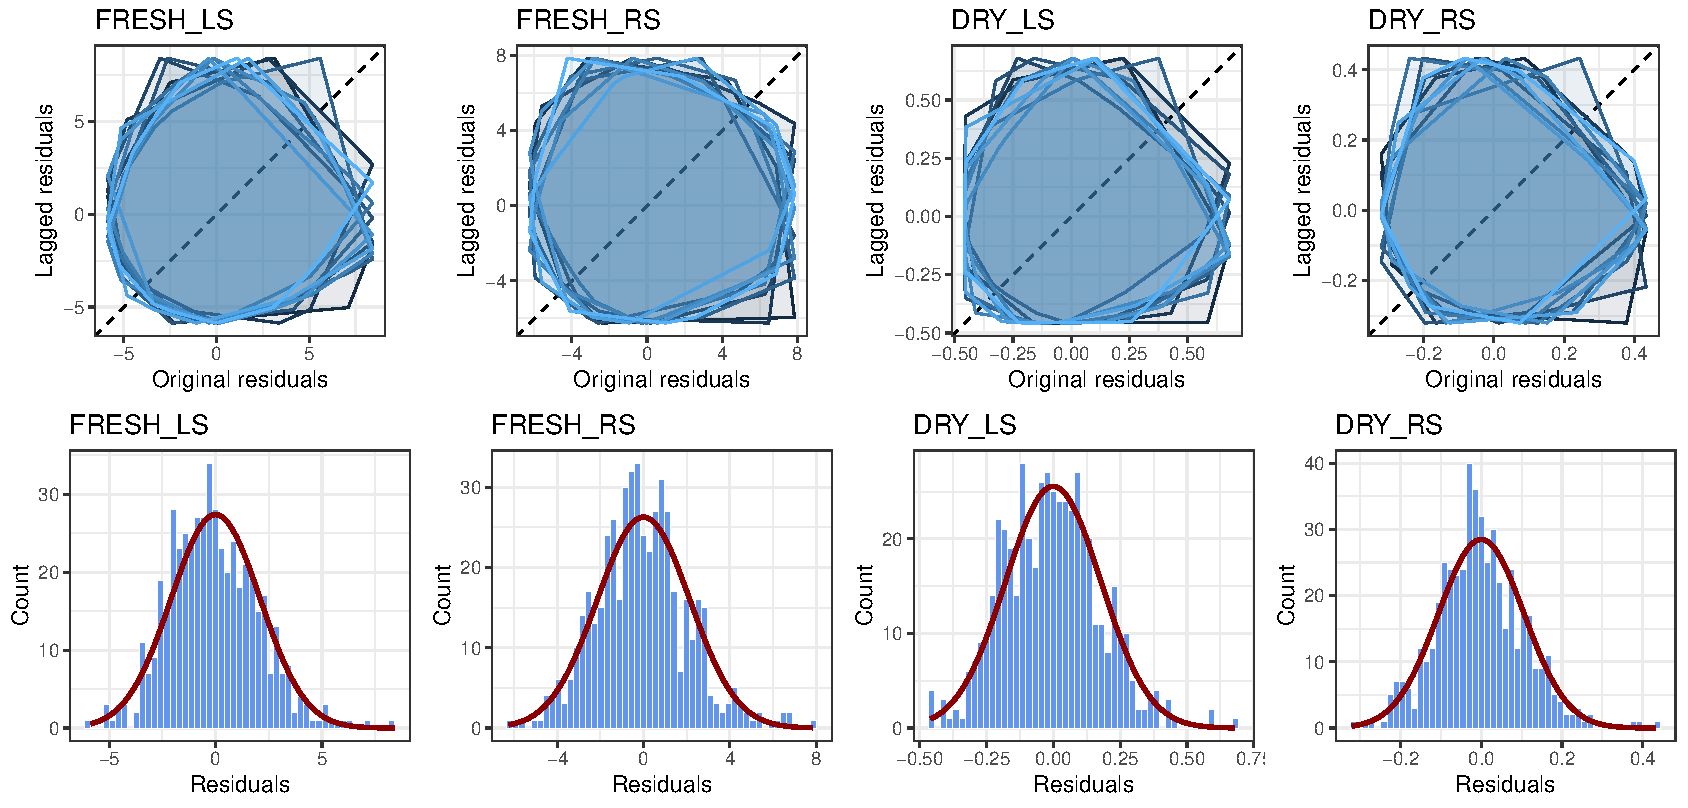
\includegraphics[width = 0.9\textwidth]{../../Figures/residuals_analysis_plot.pdf}
	\caption[Graphical analysis of the residuals og the SpATS model]{Graphical analysis of the residuals of the SpATS model for each variable: a convexhull of the lagplots of the residuals with different levels of lag (first row) and an histogram with a zero-mean, and same variance, normal distribution (second row).}
	\label{fig:residuals_analysis_plot}
\end{sidewaysfigure}

\section{Descriptive statistics}
\label{appendix:mean_std_table}

\begin{table}[ht]
\centering
\caption[Weighted mean and standard deviation for each genotype]{Weighted mean and standard deviation for each genotype. $\mathbf{DRY_{LS}}$ represents the dry weight of the leaf system; $\mathbf{DRY_{RS}}$, the dry weight for the root system; $\mathbf{FRESH_{LS}}$, the fresh weight for the leaf system and $\mathbf{FRESH_{RS}}$, the fresh weight for the root system. All the results are presented as mean $\pm$ standard deviation (g)}
\rowcolors{2}{gray!25}{white} 
\begin{tabular}{lrrrr}
  \toprule
Genotype & $DRY_{LS}$ & $DRY_{RS}$ & $FRESH_{LS}$ & $FRESH_{RS}$ \\ 
  \midrule
1 & 0.2267 $\pm$ 0.0869 & 0.2354 $\pm$ 0.0698 & 2.7231 $\pm$ 1.1612 & 3.4447 $\pm$ 1.4431 \\ 
  2 & 0.2113 $\pm$ 0.0993 & 0.1964 $\pm$ 0.06 & 2.4058 $\pm$ 1.254 & 2.2725 $\pm$ 1.1119 \\ 
  3 & 0.2132 $\pm$ 0.0747 & 0.1939 $\pm$ 0.0474 & 2.406 $\pm$ 1.0814 & 2.8146 $\pm$ 1.3663 \\ 
  4 & 0.227 $\pm$ 0.1148 & 0.1824 $\pm$ 0.0861 & 2.45 $\pm$ 1.5508 & 2.7773 $\pm$ 2.1926 \\ 
  5 & 0.2126 $\pm$ 0.113 & 0.1829 $\pm$ 0.0606 & 2.6521 $\pm$ 1.5044 & 3.0241 $\pm$ 1.7336 \\ 
  6 & 0.2024 $\pm$ 0.0739 & 0.1747 $\pm$ 0.051 & 2.4244 $\pm$ 1.1691 & 3.2168 $\pm$ 1.4545 \\ 
  7 & 0.126 $\pm$ 0.0441 & 0.1251 $\pm$ 0.0232 & 1.4118 $\pm$ 0.5677 & 1.5669 $\pm$ 0.5783 \\ 
  8 & 0.186 $\pm$ 0.0805 & 0.1798 $\pm$ 0.0567 & 2.3614 $\pm$ 1.1696 & 2.6894 $\pm$ 1.273 \\ 
  9 & 0.1559 $\pm$ 0.0865 & 0.2064 $\pm$ 0.0574 & 1.9704 $\pm$ 1.1782 & 2.3862 $\pm$ 1.3949 \\ 
  10 & 0.1885 $\pm$ 0.0875 & 0.1769 $\pm$ 0.0693 & 2.1228 $\pm$ 1.046 & 2.029 $\pm$ 1.0451 \\ 
  11 & 0.1789 $\pm$ 0.0811 & 0.1783 $\pm$ 0.0521 & 2.1608 $\pm$ 1.0747 & 2.339 $\pm$ 1.2172 \\ 
  12 & 0.1684 $\pm$ 0.0893 & 0.1469 $\pm$ 0.0417 & 2.0166 $\pm$ 0.9281 & 2.0985 $\pm$ 0.9015 \\ 
  13 & 0.1927 $\pm$ 0.0794 & 0.1639 $\pm$ 0.054 & 2.1326 $\pm$ 1.077 & 2.1176 $\pm$ 1.1582 \\ 
  14 & 0.2438 $\pm$ 0.1288 & 0.2173 $\pm$ 0.0796 & 3.0901 $\pm$ 1.6735 & 3.486 $\pm$ 1.8646 \\ 
  15 & 0.1175 $\pm$ 0.0885 & 0.2097 $\pm$ 0.0591 & 1.48 $\pm$ 1.2962 & 1.8417 $\pm$ 1.3372 \\ 
  16 & 0.3244 $\pm$ 0.1276 & 0.2208 $\pm$ 0.0879 & 3.7094 $\pm$ 1.8196 & 3.9028 $\pm$ 2.2598 \\ 
  17 & 0.2357 $\pm$ 0.1111 & 0.2019 $\pm$ 0.065 & 2.7519 $\pm$ 1.2418 & 2.8555 $\pm$ 1.4 \\ 
  18 & 0.1427 $\pm$ 0.039 & 0.1653 $\pm$ 0.0442 & 1.5621 $\pm$ 0.5627 & 1.7781 $\pm$ 0.8075 \\ 
  19 & 0.1785 $\pm$ 0.0505 & 0.1926 $\pm$ 0.04 & 2.0917 $\pm$ 0.7454 & 2.7726 $\pm$ 0.9668 \\ 
  20 & 0.1901 $\pm$ 0.0721 & 0.1506 $\pm$ 0.0497 & 2.0641 $\pm$ 0.9693 & 2.2429 $\pm$ 1.2908 \\ 
  21 & 0.1649 $\pm$ 0.0786 & 0.1859 $\pm$ 0.0329 & 1.9682 $\pm$ 0.8601 & 1.7689 $\pm$ 0.6407 \\ 
  22 & 0.1482 $\pm$ 0.0669 & 0.1508 $\pm$ 0.0296 & 1.522 $\pm$ 0.7799 & 1.793 $\pm$ 0.838 \\ 
  23 & 0.156 $\pm$ 0.04 & 0.1574 $\pm$ 0.0372 & 1.7621 $\pm$ 0.6537 & 1.9874 $\pm$ 0.9962 \\ 
  24 & 0.1668 $\pm$ 0.0827 & 0.1236 $\pm$ 0.0575 & 1.9357 $\pm$ 0.8693 & 2.0506 $\pm$ 1.2218 \\ 
  25 & 0.2013 $\pm$ 0.0856 & 0.1195 $\pm$ 0.0481 & 2.4338 $\pm$ 1.0937 & 1.9605 $\pm$ 1.1428 \\ 
  26 & 0.1463 $\pm$ 0.075 & 0.1573 $\pm$ 0.0365 & 1.7995 $\pm$ 1.1967 & 1.9256 $\pm$ 1.0053 \\ 
  27 & 0.1682 $\pm$ 0.0894 & 0.188 $\pm$ 0.0401 & 2.2662 $\pm$ 1.0855 & 2.3647 $\pm$ 1.0382 \\ 
  28 & 0.1753 $\pm$ 0.0865 & 0.2244 $\pm$ 0.066 & 2.0357 $\pm$ 1.0699 & 2.441 $\pm$ 1.1785 \\ 
  29 & 0.215 $\pm$ 0.0934 & 0.1823 $\pm$ 0.0663 & 2.4861 $\pm$ 1.3776 & 2.6743 $\pm$ 1.5787 \\ 
  30 & 0.1573 $\pm$ 0.0592 & 0.184 $\pm$ 0.0485 & 2.1033 $\pm$ 0.8712 & 2.51 $\pm$ 1.1265 \\ 
   \bottomrule
\end{tabular}
\label{tab:summary_table_all_variables}
\end{table}


\section{T-tests}
\label{appendix:t_test}
% Table generated by Excel2LaTeX from sheet 'Sheet1'
% Table generated by Excel2LaTeX from sheet 'Sheet1'
\begin{table}[htbp]
  \centering
  \caption[P-values resulting from the individual t-tests of the differences between means for all genotypes]{P-values resulting from the individual t-tests of the differences between means for all genotypes. All values inferior to 0.05 are colored in green, while value between 0.05 and 0.1 are in yellow and the rest is in red. P-value was not computed for genotype 30 since there were only 3 values available.}
    \begin{tabular}{lrrrr}
    \toprule
        Genotype  & \multicolumn{1}{l}{FRESH\_LS} & \multicolumn{1}{l}{FRESH\_RS} & \multicolumn{1}{l}{DRY\_LS} & \multicolumn{1}{l}{DRY\_LS} \\
          \bottomrule
    6     & \cellcolor[rgb]{ 1,  .922,  .612} \textcolor[rgb]{ .612,  .341,  0}{0,067045} & \cellcolor[rgb]{ .776,  .937,  .808} \textcolor[rgb]{ 0,  .38,  0}{8,18E-05} & \cellcolor[rgb]{ .776,  .937,  .808} \textcolor[rgb]{ 0,  .38,  0}{0,024774} & \cellcolor[rgb]{ .776,  .937,  .808} \textcolor[rgb]{ 0,  .38,  0}{0,000941} \\
    23    & \cellcolor[rgb]{ .776,  .937,  .808} \textcolor[rgb]{ 0,  .38,  0}{0,005072} & \cellcolor[rgb]{ .776,  .937,  .808} \textcolor[rgb]{ 0,  .38,  0}{0,009236} & \cellcolor[rgb]{ 1,  .922,  .612} \textcolor[rgb]{ .612,  .341,  0}{0,076901} & \cellcolor[rgb]{ .776,  .937,  .808} \textcolor[rgb]{ 0,  .38,  0}{0,036332} \\
    10    & \cellcolor[rgb]{ .776,  .937,  .808} \textcolor[rgb]{ 0,  .38,  0}{0,007526} & \cellcolor[rgb]{ .776,  .937,  .808} \textcolor[rgb]{ 0,  .38,  0}{0,001057} & \cellcolor[rgb]{ 1,  .78,  .808} \textcolor[rgb]{ .612,  0,  .024}{0,10752} & \cellcolor[rgb]{ 1,  .922,  .612} \textcolor[rgb]{ .612,  .341,  0}{0,054917} \\
    26    & \cellcolor[rgb]{ 1,  .922,  .612} \textcolor[rgb]{ .612,  .341,  0}{0,068053} & \cellcolor[rgb]{ .776,  .937,  .808} \textcolor[rgb]{ 0,  .38,  0}{0,029225} & \cellcolor[rgb]{ 1,  .922,  .612} \textcolor[rgb]{ .612,  .341,  0}{0,092141} & \cellcolor[rgb]{ .776,  .937,  .808} \textcolor[rgb]{ 0,  .38,  0}{0,007438} \\
    4     & \cellcolor[rgb]{ .776,  .937,  .808} \textcolor[rgb]{ 0,  .38,  0}{0,034853} & \cellcolor[rgb]{ .776,  .937,  .808} \textcolor[rgb]{ 0,  .38,  0}{0,024024} & \cellcolor[rgb]{ 1,  .78,  .808} \textcolor[rgb]{ .612,  0,  .024}{0,109144} & \cellcolor[rgb]{ .776,  .937,  .808} \textcolor[rgb]{ 0,  .38,  0}{0,032899} \\
    8     & \cellcolor[rgb]{ .776,  .937,  .808} \textcolor[rgb]{ 0,  .38,  0}{0,009049} & \cellcolor[rgb]{ .776,  .937,  .808} \textcolor[rgb]{ 0,  .38,  0}{0,00777} & \cellcolor[rgb]{ .776,  .937,  .808} \textcolor[rgb]{ 0,  .38,  0}{0,035141} & \cellcolor[rgb]{ 1,  .78,  .808} \textcolor[rgb]{ .612,  0,  .024}{0,201765} \\
    14    & \cellcolor[rgb]{ .776,  .937,  .808} \textcolor[rgb]{ 0,  .38,  0}{0,04338} & \cellcolor[rgb]{ .776,  .937,  .808} \textcolor[rgb]{ 0,  .38,  0}{0,023285} & \cellcolor[rgb]{ 1,  .78,  .808} \textcolor[rgb]{ .612,  0,  .024}{0,256493} & \cellcolor[rgb]{ 1,  .922,  .612} \textcolor[rgb]{ .612,  .341,  0}{0,09208} \\
    9     & \cellcolor[rgb]{ .776,  .937,  .808} \textcolor[rgb]{ 0,  .38,  0}{0,038485} & \cellcolor[rgb]{ .776,  .937,  .808} \textcolor[rgb]{ 0,  .38,  0}{0,039673} & \cellcolor[rgb]{ 1,  .78,  .808} \textcolor[rgb]{ .612,  0,  .024}{0,220818} & \cellcolor[rgb]{ 1,  .78,  .808} \textcolor[rgb]{ .612,  0,  .024}{0,123382} \\
    24    & \cellcolor[rgb]{ .776,  .937,  .808} \textcolor[rgb]{ 0,  .38,  0}{0,042817} & \cellcolor[rgb]{ .776,  .937,  .808} \textcolor[rgb]{ 0,  .38,  0}{0,015859} & \cellcolor[rgb]{ 1,  .78,  .808} \textcolor[rgb]{ .612,  0,  .024}{0,408412} & \cellcolor[rgb]{ 1,  .922,  .612} \textcolor[rgb]{ .612,  .341,  0}{0,079817} \\
    3     & \cellcolor[rgb]{ 1,  .922,  .612} \textcolor[rgb]{ .612,  .341,  0}{0,07032} & \cellcolor[rgb]{ .776,  .937,  .808} \textcolor[rgb]{ 0,  .38,  0}{0,020974} & \cellcolor[rgb]{ 1,  .78,  .808} \textcolor[rgb]{ .612,  0,  .024}{0,492672} & \cellcolor[rgb]{ 1,  .922,  .612} \textcolor[rgb]{ .612,  .341,  0}{0,060329} \\
    29    & \cellcolor[rgb]{ 1,  .922,  .612} \textcolor[rgb]{ .612,  .341,  0}{0,066428} & \cellcolor[rgb]{ 1,  .922,  .612} \textcolor[rgb]{ .612,  .341,  0}{0,055044} & \cellcolor[rgb]{ 1,  .78,  .808} \textcolor[rgb]{ .612,  0,  .024}{0,348994} & \cellcolor[rgb]{ 1,  .78,  .808} \textcolor[rgb]{ .612,  0,  .024}{0,183319} \\
    25    & \cellcolor[rgb]{ 1,  .922,  .612} \textcolor[rgb]{ .612,  .341,  0}{0,086712} & \cellcolor[rgb]{ .776,  .937,  .808} \textcolor[rgb]{ 0,  .38,  0}{0,013015} & \cellcolor[rgb]{ 1,  .78,  .808} \textcolor[rgb]{ .612,  0,  .024}{0,564199} & \cellcolor[rgb]{ 1,  .922,  .612} \textcolor[rgb]{ .612,  .341,  0}{0,091173} \\
    16    & \cellcolor[rgb]{ .776,  .937,  .808} \textcolor[rgb]{ 0,  .38,  0}{0,015628} & \cellcolor[rgb]{ .776,  .937,  .808} \textcolor[rgb]{ 0,  .38,  0}{0,002877} & \cellcolor[rgb]{ 1,  .78,  .808} \textcolor[rgb]{ .612,  0,  .024}{0,637848} & \cellcolor[rgb]{ 1,  .78,  .808} \textcolor[rgb]{ .612,  0,  .024}{0,164959} \\
    27    & \cellcolor[rgb]{ 1,  .922,  .612} \textcolor[rgb]{ .612,  .341,  0}{0,068433} & \cellcolor[rgb]{ .776,  .937,  .808} \textcolor[rgb]{ 0,  .38,  0}{0,001215} & \cellcolor[rgb]{ 1,  .78,  .808} \textcolor[rgb]{ .612,  0,  .024}{0,728604} & \cellcolor[rgb]{ .776,  .937,  .808} \textcolor[rgb]{ 0,  .38,  0}{0,036351} \\
    15    & \cellcolor[rgb]{ 1,  .78,  .808} \textcolor[rgb]{ .612,  0,  .024}{0,249287} & \cellcolor[rgb]{ 1,  .78,  .808} \textcolor[rgb]{ .612,  0,  .024}{0,264329} & \cellcolor[rgb]{ 1,  .78,  .808} \textcolor[rgb]{ .612,  0,  .024}{0,299309} & \cellcolor[rgb]{ 1,  .78,  .808} \textcolor[rgb]{ .612,  0,  .024}{0,383055} \\
    18    & \cellcolor[rgb]{ 1,  .78,  .808} \textcolor[rgb]{ .612,  0,  .024}{0,25502} & \cellcolor[rgb]{ 1,  .922,  .612} \textcolor[rgb]{ .612,  .341,  0}{0,054048} & \cellcolor[rgb]{ 1,  .78,  .808} \textcolor[rgb]{ .612,  0,  .024}{0,806946} & \cellcolor[rgb]{ 1,  .78,  .808} \textcolor[rgb]{ .612,  0,  .024}{0,14867} \\
    13    & \cellcolor[rgb]{ 1,  .78,  .808} \textcolor[rgb]{ .612,  0,  .024}{0,278165} & \cellcolor[rgb]{ 1,  .78,  .808} \textcolor[rgb]{ .612,  0,  .024}{0,130413} & \cellcolor[rgb]{ 1,  .78,  .808} \textcolor[rgb]{ .612,  0,  .024}{0,634507} & \cellcolor[rgb]{ 1,  .78,  .808} \textcolor[rgb]{ .612,  0,  .024}{0,287053} \\
    5     & \cellcolor[rgb]{ 1,  .78,  .808} \textcolor[rgb]{ .612,  0,  .024}{0,112019} & \cellcolor[rgb]{ .776,  .937,  .808} \textcolor[rgb]{ 0,  .38,  0}{0,047269} & \cellcolor[rgb]{ 1,  .78,  .808} \textcolor[rgb]{ .612,  0,  .024}{0,439077} & \cellcolor[rgb]{ 1,  .78,  .808} \textcolor[rgb]{ .612,  0,  .024}{0,742416} \\
    12    & \cellcolor[rgb]{ 1,  .78,  .808} \textcolor[rgb]{ .612,  0,  .024}{0,302533} & \cellcolor[rgb]{ 1,  .78,  .808} \textcolor[rgb]{ .612,  0,  .024}{0,792875} & \cellcolor[rgb]{ 1,  .922,  .612} \textcolor[rgb]{ .612,  .341,  0}{0,051195} & \cellcolor[rgb]{ 1,  .78,  .808} \textcolor[rgb]{ .612,  0,  .024}{0,271333} \\
    1     & \cellcolor[rgb]{ .776,  .937,  .808} \textcolor[rgb]{ 0,  .38,  0}{0,027344} & \cellcolor[rgb]{ .776,  .937,  .808} \textcolor[rgb]{ 0,  .38,  0}{0,004086} & \cellcolor[rgb]{ 1,  .78,  .808} \textcolor[rgb]{ .612,  0,  .024}{0,93751} & \cellcolor[rgb]{ 1,  .78,  .808} \textcolor[rgb]{ .612,  0,  .024}{0,512452} \\
    20    & \cellcolor[rgb]{ 1,  .78,  .808} \textcolor[rgb]{ .612,  0,  .024}{0,178574} & \cellcolor[rgb]{ 1,  .78,  .808} \textcolor[rgb]{ .612,  0,  .024}{0,110094} & \cellcolor[rgb]{ 1,  .78,  .808} \textcolor[rgb]{ .612,  0,  .024}{0,943514} & \cellcolor[rgb]{ 1,  .78,  .808} \textcolor[rgb]{ .612,  0,  .024}{0,447728} \\
    19    & \cellcolor[rgb]{ 1,  .78,  .808} \textcolor[rgb]{ .612,  0,  .024}{0,170245} & \cellcolor[rgb]{ .776,  .937,  .808} \textcolor[rgb]{ 0,  .38,  0}{0,038213} & \cellcolor[rgb]{ 1,  .78,  .808} \textcolor[rgb]{ .612,  0,  .024}{0,684042} & \cellcolor[rgb]{ 1,  .78,  .808} \textcolor[rgb]{ .612,  0,  .024}{0,87518} \\
    7     & \cellcolor[rgb]{ 1,  .78,  .808} \textcolor[rgb]{ .612,  0,  .024}{0,119486} & \cellcolor[rgb]{ .776,  .937,  .808} \textcolor[rgb]{ 0,  .38,  0}{0,017251} & \cellcolor[rgb]{ 1,  .78,  .808} \textcolor[rgb]{ .612,  0,  .024}{0,915835} & \cellcolor[rgb]{ 1,  .78,  .808} \textcolor[rgb]{ .612,  0,  .024}{0,878908} \\
    28    & \cellcolor[rgb]{ 1,  .78,  .808} \textcolor[rgb]{ .612,  0,  .024}{0,360779} & \cellcolor[rgb]{ 1,  .78,  .808} \textcolor[rgb]{ .612,  0,  .024}{0,127756} & \cellcolor[rgb]{ 1,  .78,  .808} \textcolor[rgb]{ .612,  0,  .024}{0,954177} & \cellcolor[rgb]{ 1,  .78,  .808} \textcolor[rgb]{ .612,  0,  .024}{0,606738} \\
    21    & \cellcolor[rgb]{ 1,  .78,  .808} \textcolor[rgb]{ .612,  0,  .024}{0,574376} & \cellcolor[rgb]{ 1,  .78,  .808} \textcolor[rgb]{ .612,  0,  .024}{0,503482} & \cellcolor[rgb]{ 1,  .78,  .808} \textcolor[rgb]{ .612,  0,  .024}{0,42371} & \cellcolor[rgb]{ 1,  .78,  .808} \textcolor[rgb]{ .612,  0,  .024}{0,570469} \\
    2     & \cellcolor[rgb]{ 1,  .78,  .808} \textcolor[rgb]{ .612,  0,  .024}{0,453042} & \cellcolor[rgb]{ 1,  .922,  .612} \textcolor[rgb]{ .612,  .341,  0}{0,077753} & \cellcolor[rgb]{ 1,  .78,  .808} \textcolor[rgb]{ .612,  0,  .024}{0,790318} & \cellcolor[rgb]{ 1,  .78,  .808} \textcolor[rgb]{ .612,  0,  .024}{0,828287} \\
    11    & \cellcolor[rgb]{ 1,  .78,  .808} \textcolor[rgb]{ .612,  0,  .024}{0,875426} & \cellcolor[rgb]{ 1,  .78,  .808} \textcolor[rgb]{ .612,  0,  .024}{0,772947} & \cellcolor[rgb]{ 1,  .78,  .808} \textcolor[rgb]{ .612,  0,  .024}{0,404975} & \cellcolor[rgb]{ 1,  .78,  .808} \textcolor[rgb]{ .612,  0,  .024}{0,179616} \\
    22    & \cellcolor[rgb]{ 1,  .78,  .808} \textcolor[rgb]{ .612,  0,  .024}{0,793643} & \cellcolor[rgb]{ 1,  .78,  .808} \textcolor[rgb]{ .612,  0,  .024}{0,55334} & \cellcolor[rgb]{ 1,  .78,  .808} \textcolor[rgb]{ .612,  0,  .024}{0,510492} & \cellcolor[rgb]{ 1,  .78,  .808} \textcolor[rgb]{ .612,  0,  .024}{0,40223} \\
    17    & \cellcolor[rgb]{ 1,  .78,  .808} \textcolor[rgb]{ .612,  0,  .024}{0,887499} & \cellcolor[rgb]{ 1,  .78,  .808} \textcolor[rgb]{ .612,  0,  .024}{0,192592} & \cellcolor[rgb]{ 1,  .78,  .808} \textcolor[rgb]{ .612,  0,  .024}{0,493846} & \cellcolor[rgb]{ 1,  .78,  .808} \textcolor[rgb]{ .612,  0,  .024}{0,835214} \\
    30    & . & . & . & . \\
    \midrule
    \end{tabular}%
  \label{tab:ind_geno_t_test_pval}%
\end{table}%




\section{Variance tables}
\subsection{SpATS variance table}
\label{appendix:tab_spats_variances}

\begin{table}[ht]
\centering
\rowcolors{2}{gray!25}{white}
\caption{Individual variances of all the components of the SpATS model.} 
\begin{tabular}{lrrrr}
  \toprule
 & FRESH\_LS & FRESH\_RS & DRY\_LS & DRY\_RS \\ 
  \midrule
$\mathbf{c}_{g}$ & 0.171 & 0.262 & 1.27$\times 10^{-3}$ & 6.9$\times 10^{-4}$ \\ 
  $\mathbf{c}_{v}$ & 3.24$\times 10^{-3}$ & 5.08$\times 10^{-3}$ & 1.95$\times 10^{-7}$ & 8.47$\times 10^{-17}$ \\ 
  $\mathbf{c}_{u}$ & 1.86$\times 10^{-4}$ & 2.25$\times 10^{-5}$ & 2.42$\times 10^{-7}$ & 3.93$\times 10^{-8}$ \\ 
  $f_{v}(\mathbf{v})$ & 2.2 & 11 & 1.06$\times 10^{-4}$ & 0.265 \\ 
  $f_{u}(\mathbf{u})$ & 2.75$\times 10^{-5}$ & 5.36$\times 10^{-5}$ & 5.4$\times 10^{-8}$ & 1.55$\times 10^{-8}$ \\ 
  $\boldsymbol{u} \odot h_{v}(\boldsymbol{v})$ & 5.60$\times 10^{-52}$ & 1.76$\times 10^{-38}$ & 1.51$\times 10^{-52}$ & 1.44$\times 10^{-13}$ \\ 
  $\boldsymbol{v} \odot h_{u}(\boldsymbol{u})$ & 1.81$\times 10^{-9}$ & 4.83$\times 10^{-4}$ & 6.75$\times 10^{-10}$ & 1.43$\times 10^{-6}$ \\ 
  $f_{u, v}(\boldsymbol{u}, \boldsymbol{v})$ & 0.398 & 0.252 & 6.13$\times 10^{-5}$ & 7.13$\times 10^{-4}$ \\ 
  $\epsilon$ & 4.707 & 5.014 & 0.03364 & 0.01219\\
   \bottomrule
\end{tabular}
\label{tab:spats_variances}
\end{table}

%\chapter{Hoagland solution}
%\label{appendix:hoagland}
%
%\rowcolors{2}{gray!25}{white}
%
%\captionsetup[table]{list=no}
%\begin{table}[hbtp]
%    \centering
%    \caption{Composition of the \textit{Hoagland} nutritive solution. The pH must be adjusted to 5.0 using \ch{HCl} 1\% before using.}
%    \label{tab:my_label}
%    \begin{threeparttable}
%    \begin{tabular}{>{\bfseries}p{4cm} p{4cm} p{4cm}}
%    \toprule
%        Components & \textbf{Concentration (g/L)} & \textbf{ml for 25L of solution}\tnote{1} \\
%    \midrule
%        2M \ch{KNO3} & 202 & 62.5 \\
%        2M \ch{Ca(NO3)2} x \ch{4 H2O}  & 472 & 62.5\\
%        2M \ch{MgSO4} x \ch{7 H2O} & 493 & 25\\
%        1M \ch{NH4NO3} & 80 & 25\\
%        Minors: \newline
%        \ch{H3BO3} \newline
%        \ch{MnCl2} x \ch{4 H2O} \newline
%        \ch{ZnSO4} x \ch{7 H2O} \newline
%        \ch{CuSO4} \newline
%        \ch{H3MoO4} x \ch{H2O} or \newline
%        \ch{Na2MoO4} x \ch{2 H2O} & 
%        ~    \newline
%        2.86 \newline
%        1.81 \newline
%        0.22 \newline
%        0.051 \newline
%        0.09 \newline 
%        0.12 & 
%        ~    \newline
%        ~    \newline
%        ~    \newline
%        25 \tnote{2} \\
%        1M \ch{KH2PO4} (ph to 6.0 with 3M \ch{KOH}) & 136 & 12.5\\
%        Iron (Sprint 138 iron chelate) & 15 & 75\\
%    \bottomrule
%    \end{tabular}
%    \begin{tablenotes}\footnotesize
%        \item[1] For a 1:1 solution to use with 25L of water.
%        \item[2] All the minors elements are grouped, in the right proportions, in a "minor" solution.
%    \end{tablenotes}
%    \end{threeparttable}
%\end{table}
%\captionsetup[table]{list=yes}

\chapter{Phenotyping platform information file}
\label{appendix:platform_info}
\clearpage
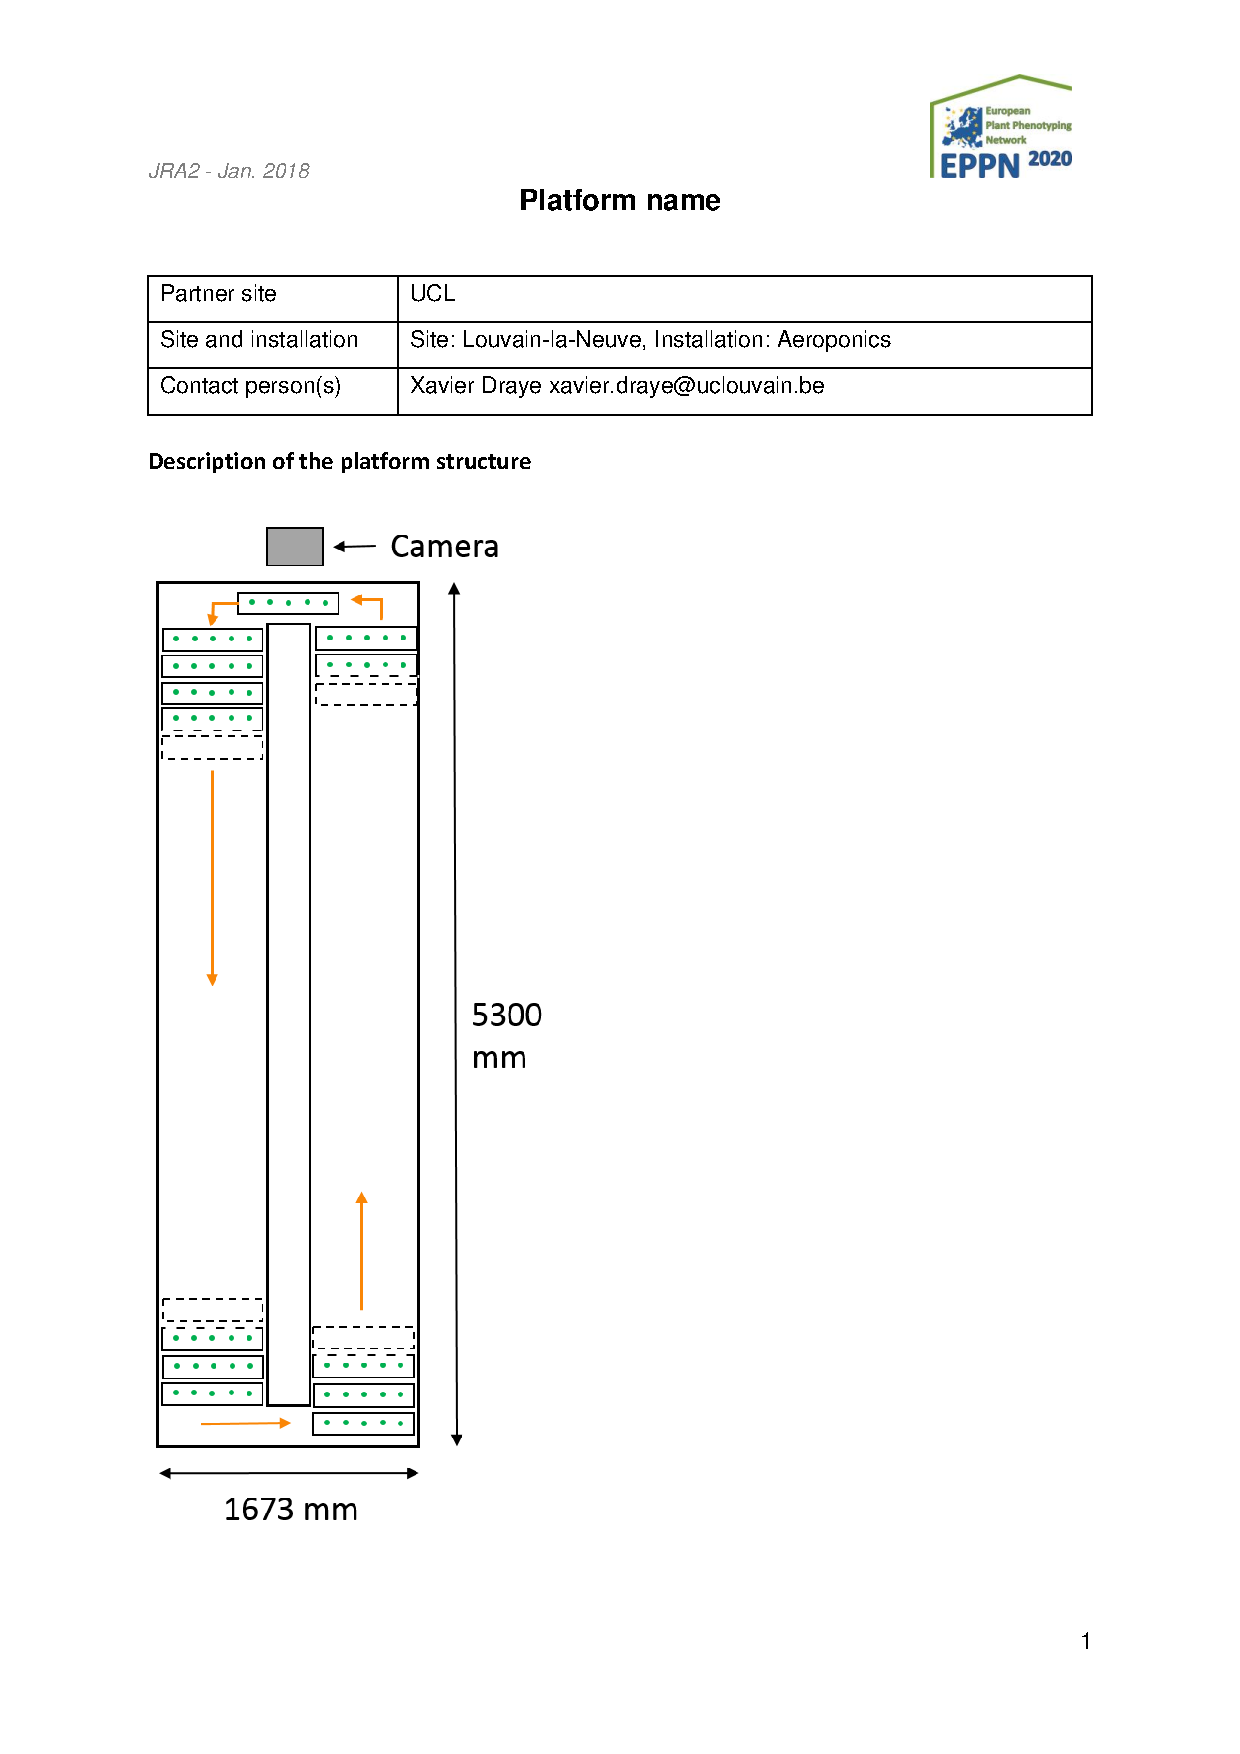
\includepdf[pages=-,pagecommand={},width=\textwidth]{extra/platform_info.pdf}
